\documentclass[12pt]{article}
\usepackage{graphicx}
\graphicspath{ {./InterpretEEGWayneImages/} }

\title{EEG (electroencephalogram)}
\author{Annabelle Chan}
\date{September 2024}

\begin{document}
\maketitle
Link: https://neurology.med.wayne.edu/pdfs/how\_to\_interpret\_and\_eeg\_and\_its\_report.pdf

Author: Marie Atkinson (Wayne university medical school, Comprehensive Epilepsy Program)

Date: July 19, 2010

\section{Managing an EEG Scan}
Sensitivity is represented by the amplitudes of the wave lines from the scan. The lower the voltage used (in microvolts) the larger of the amplitude, the more you will see on the scan. It's usually around 7.5 microvolts.
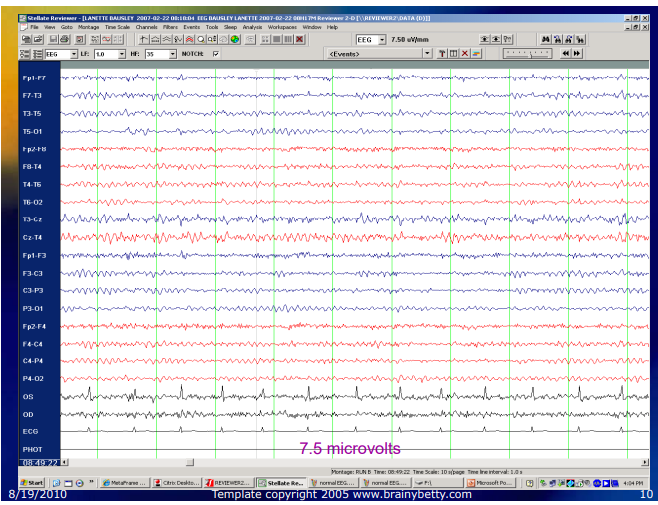
\includegraphics[scale=0.5]{lowSensitivity}
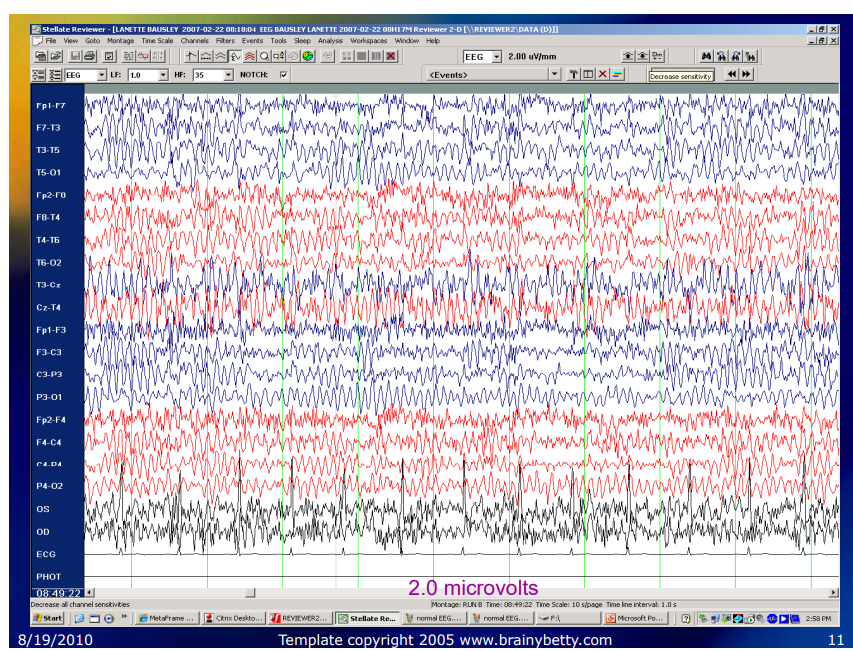
\includegraphics[scale=0.4]{highSensitivity}
\medskip
	An EEG Scan can have 3 different filters:

	Low Frequency (LF) Filter:  If you set a frequency at frequency x, eeg will not amplify any frequencies below that number. It's usually set at 1.0 Hz.

	High Frequency (HF) Filter: If you set a frequency at frequency x, eeg will not amplify any frequencies above that number. It's usually set at 35 Hz

	Notch Filter: It cuts off any activity above and at 60 Hz. The current through plugs is often at 60 Hz and allows people to ignore outside artifacts by other machinery in the room.
 
\section{Background activity}
Just based on the frequency (delta, theta, alpha, or beta), we get an overall sense on how the person being tested is doing.

Deta 1-3 Hz: Marked slowing

Theta 4-7 Hz: Mildly slow 

Alpha 8-13 Hz: Normal background

Beta (above 13 Hz): Barbiturates/Benzos (sedating drugs https://www.ncbi.nlm.nih.gov/books/NBK390343/.)
\medskip
	It's Usually evaluated in the posterior channel (back part of the complete cerebral cortex) and often in occipital (visual processing area of the brain within the posterior channel). The person being tested must have their eyes closed.

\section{Symmetry}

Asymmetric slowing is seen with focal lesions, surgery, etc. and easiest to see with A montage. It can be seen by hyperventilation or photic stimulation.
 
PLEDs (Periodic Lateralized Epileptiform Discharges) occurs throughout the entire EEG at a frequency of 1-2 Hz and only in one hemisphere. It is usually seen in acute lesions (stroke, bleed, etc.), postictal, Herpes Encephalitis, CJD, and etc. Its reading meaning is controversial (because it's thought to be inconclusive?)

\section{Abnormality classifications}

Epileptiform Activity means the EEG reader saw some abnormalities that is related to seizures (but needs clinical correlation). These abnormalities include sharp waves, spikes, or slow waves. 

Spikes are abnormal wave lasting 70 microvolts or less. It stands out from the background. On a Bipolar Montage, it needs to have phase reversal to be real. 

Sharp Wave last about 70-200 microvolts. It also stands out from the background and on a Bipolar Montage, it needs to have phase reversal to be real. Both sides of the slope should be sloped. If it’s straight on one side, it’s usually an artifact (a noise or disturbance in the data not from the brain). 

Slow Waves last greater than 200 microvolts, and it also stands out from the background.
\medskip
	For actual seizures, the EEG reader can tell if it’s partial or generalized, status epilepticus, or consistent with primary generalized syndrome. A seizure should be like a wave, and have a buildup and let down
\medskip
	Triphasic waves usually indicates metabolic or toxic encephalopathy (usually liver failure or renal disease). Patients always have some degree of encephalopathy (mild to moderate). It can also be seen with Cefepime encephalopathy and Li intoxication and is usually anterior dominant, diffuse, and bilaterally synchronous. It has 3 phases to the waveform: negative, positive, negative and will have a lag anterior to posterior in wave 2 peak

“Looks like a backward check mark” - Guru Dr. Shah
\medskip
Primary generalized epilepsy is eneralized bursts of activity. Secondary generalized bisynchrony is a generalized burst following a localized focal abnormal epileptiform waveform (not primary generalized epilepsy).
\medskip
When a burst suppression is spontaneous, it results in a very poor prognosis.
\medskip
To pronounce someone brain dead/electrocerebral silence a specialized eeg protocol is performed. It's not performed very often due to the required time period and artifacts that may be mistaken for brain activity
\medskip
Breech rhythm is seen over a skull defect, namely surgery and has the same frequency as rest of EEG (with a higher amplitude)
\medskip
Hypsarrhythmia is seen in infantile spasms (West Syndrome) with a “chaotic” background. It will have a decremental appearance when child is actually having a spasm 
\medskip
SSPE (Subacute Sclerosing Panencephalitis) exhibits encephalitis that tends to affect young boys after experiencing measles illness. Mortality is high and those that survived have intellectual sequelae. The pattern is different from burst suppression because in between bursts, the background is not suppressed.

\section{Artifacts}
An eye blink artifact is only seen in prefrontal channels. If you look at the eye channel, the waveform occurs at the same time just in opposite directions
\medskip
The muscle artifact appears to be too sharp and usually occurs when patient is agitated or moving. If the HF filter is removed, the results get even worse
\medskip
The EKG artifact corresponds with the QRS complex on the EKG and usually looks like regular spikes transmitted throughout the EEG.
\medskip
Stages of sleep are often mistaken as abnormal and best seen on bipolar montage in Cz channels (K complexes, Vertex waves, Spindles).

\section{Normal EEG Scan}
A normal EEG should have alpha frequency background activity, no abnormalities (nothing stands out in the background), no changes in the EEG provoked by photic, hyperventilation, and no asymmetry  

\section{Terminology} 
	Epileptiform - waveforms are seen that have the potential to cause seizures but clinical correlation still needed
\medskip

	Photic Stimulation - provoking procedure done to induce primary generalized epilepsy or asymmetries 
\medskip

	Driving response - patient reacting normally to the stimulation 
\medskip

	No driving response - no EEG change with photic stimulation 
\medskip

	Hyperventilation - procedure performed to provoke primary generalized epilepsy and provoke asymmetrics. Symmetric physiological slowing is normal 
\medskip

	Stage 1 sleep - presence of vertex waves and theta slowing during EEG
\medskip

	Stage 2 sleep - presence of K complexes and sleep spindles with delta slowing during EEG
\medskip

	Drowsiness provoke epileptiform activity (the reason why sleep deprived EEG is recommended to truly rule out seizure disorder)
\medskip

	Diffuse slowing - background is theta or delta frequency. It’s seen with encephalopathic state, medication effect, prostical, dementia, and bilateral structural defect
\medskip

	Focal slowing - seen over lesions like tumors, stroke, hippocampal sclerosis, usually indicates structural lesion in area. If the patient is seizing, the report will say seizure or status epilepticus 

\end{document}




